\documentclass{article}

\usepackage{amssymb}
\usepackage{amsmath}

\title{ME699 Final Project Proposal}
\date{02-04-2020}
\author{Benton Clark, Ethan Howell, Brian Moberly}

\begin{document}
\pagenumbering{gobble}
\maketitle

\section{Project Outline}
For our project, we are proposing three primary phases:

\begin{itemize}
  \item Modeling
  \item Perception and Planning
  \item Control
\end{itemize}

\noindent Each phase of the project will feed into the next.
For instance, the model designed in the robotic modeling section will then be
used in the control section of the project.
By the end of the project, our goal is to have a fully modeled, controlled
robotic manipulator capable of following a simple trajectory and moving to
desired target locations in task space to accomplish simple goals.

\section{Demonstration}
The end goal of our project is to apply the modeling, perception and adaptive
controls to the Panda Robot arm.
The task will consist of the arm beginning in a configuration, moving towards an
intermediate state where an object is located, picking up that object, and
successfully moving that object to a desired goal state.
The object will be of unknown and variable mass, meaning the arm must be able to
effectively adapt to objects of differing weight online.
The exact location of the object must also be identified by the ``camera''
attached to the Panda, meaning a valid path must be found to both reach the
object and take it to the goal state.
The goal state will be fixed.

For the modeling portion, both static free and dry friction models will be used.
The perception and planning portion will be tasked with filtering out small
amounts of Gaussian white noise from both the joint configurations and the
camera readings in task space.
It must also find a valid trajectory of configurations in both task and joint
space to complete the objective.
The adaptive controller will use both the modeling and perception values in
determining the joint torques to command to follow the given trajectory.
It will also compensate for the additional weight on the last link of the arm
when the object of unknown mass is picked up.

\subsection*{Mass Matrix Modeling}
Modeling the mass matrix of a robotic manipulator becomes increasingly difficult as the DOF of the system increase.
Our attempt to avoid this complexity was to model the mass matrix with a neural network.
To further decrease the dimensionality of the problem, it is well understood that the mass matrix is a positive definite (PD) square matrix.
Thus the neural network output only the lower triangle of the matrix, and the remaining values were copied from the output accordingly.
Once the mass matrix neural network was trained, it was used in simulation to develop a trajectory tracking controller.

\subsection*{The Kalman Filter}
The Kalman Filter is used to mitigate the noise present in a system as the system moves.  The goal is to know what the robot is doing at the next time step, using the knowledge of the current time step.  The motion of the system is described by the following uncertainty model:
\begin{equation}
    x_{t=1}=Ax_t+Bu_t+v_t,
\end{equation}
where $v_t$ is a Gaussian noise variable pertaining to the uncertainty in the system behavior.
\\
The measurement made by the camera follows the uncertainty model
\begin{equation}
    y_t=Cx_t+w_t,
\end{equation}
where $w_t$ is a Gaussian noise variable describing the uncertainty in the camera's mapping of the environment.
\\
The Kalman Filter proceeds with a motion update that represents the motion of the model with noise:
\begin{equation}
    \mu_t^{pred}=A\mu_t+Bu_t
\end{equation}
\begin{equation}
    \Sigma_t^{pred}=A\Sigma_tA^T+R_v
\end{equation}
\\
After completing the motion, the camera makes a measurement update:
\begin{equation}
    K_t=\Sigma_t^{pred}C^{T}(C\Sigma_t^{pred}C^{T}+R_w)^{-1}
\end{equation}
\begin{equation}
    \mu_{t+1}=\mu_t^{pred}+K(y_t-C\mu_t^{pred})
\end{equation}
\begin{equation}
    \Sigma_{t+1}=(I-KC)\Sigma_t^{pred}
\end{equation}
\subsection*{Implementation}
Since the camera is attached to the end-effector, the measurements from the camera are made from the frame of the end-effector.  Since the system explores $\mathbb{R}^{3\times3}$, the Kalman Filter is created to handle three-dimensional space, ignoring orientations.  So, the robot $r$ and any landmark $L$ $\in\mathbb{R}^{3\times3}$.  The state is therefore a vector consisting of the robot and landmark x-y-z coordinates:
\begin{equation}
    x=\begin{bmatrix} x_r\\y_r\\z_r\\...\\L_{xi}\\L_{yi}\\L_{zi} \end{bmatrix}
\end{equation}
for i landmarks.
\\
Matrices A and B contain only non-zero elements on the main diagonal with entries of 1.  Matrix A has size $(3+3i)x(3+3i)$ and Matrix B is of size $(3+3i)x3$.  The matrix C describes the measurement as the distance between the landmark and the robot.  C is of size $(3i)x(3i+3)$.  The non-zero entries lie on the diagonals, with -1 entered on the corresponding robot state and 1 entered on the corresponding landmark state.
\subsection*{Control Model}
In order to implement the adaptive control in the Julia programming language, we needed a way to account for the adaptation law. This implementation was not initially very straightforward, as the ``simulate!()" function places certain restrictions on the inputs to the control function that we choose. To alleviate this issue, we made the adaptive controller a mutable structure which contains the adaptation parameter as a member. This implementation allows us to continually update the parameter, without having to troubleshoot issues associated with other methods.\\

With this control fully implemented, we then move to the full simulation of the control in which we track the state error and end-effector trajectory.
\begin{figure}[H]
	\centering
	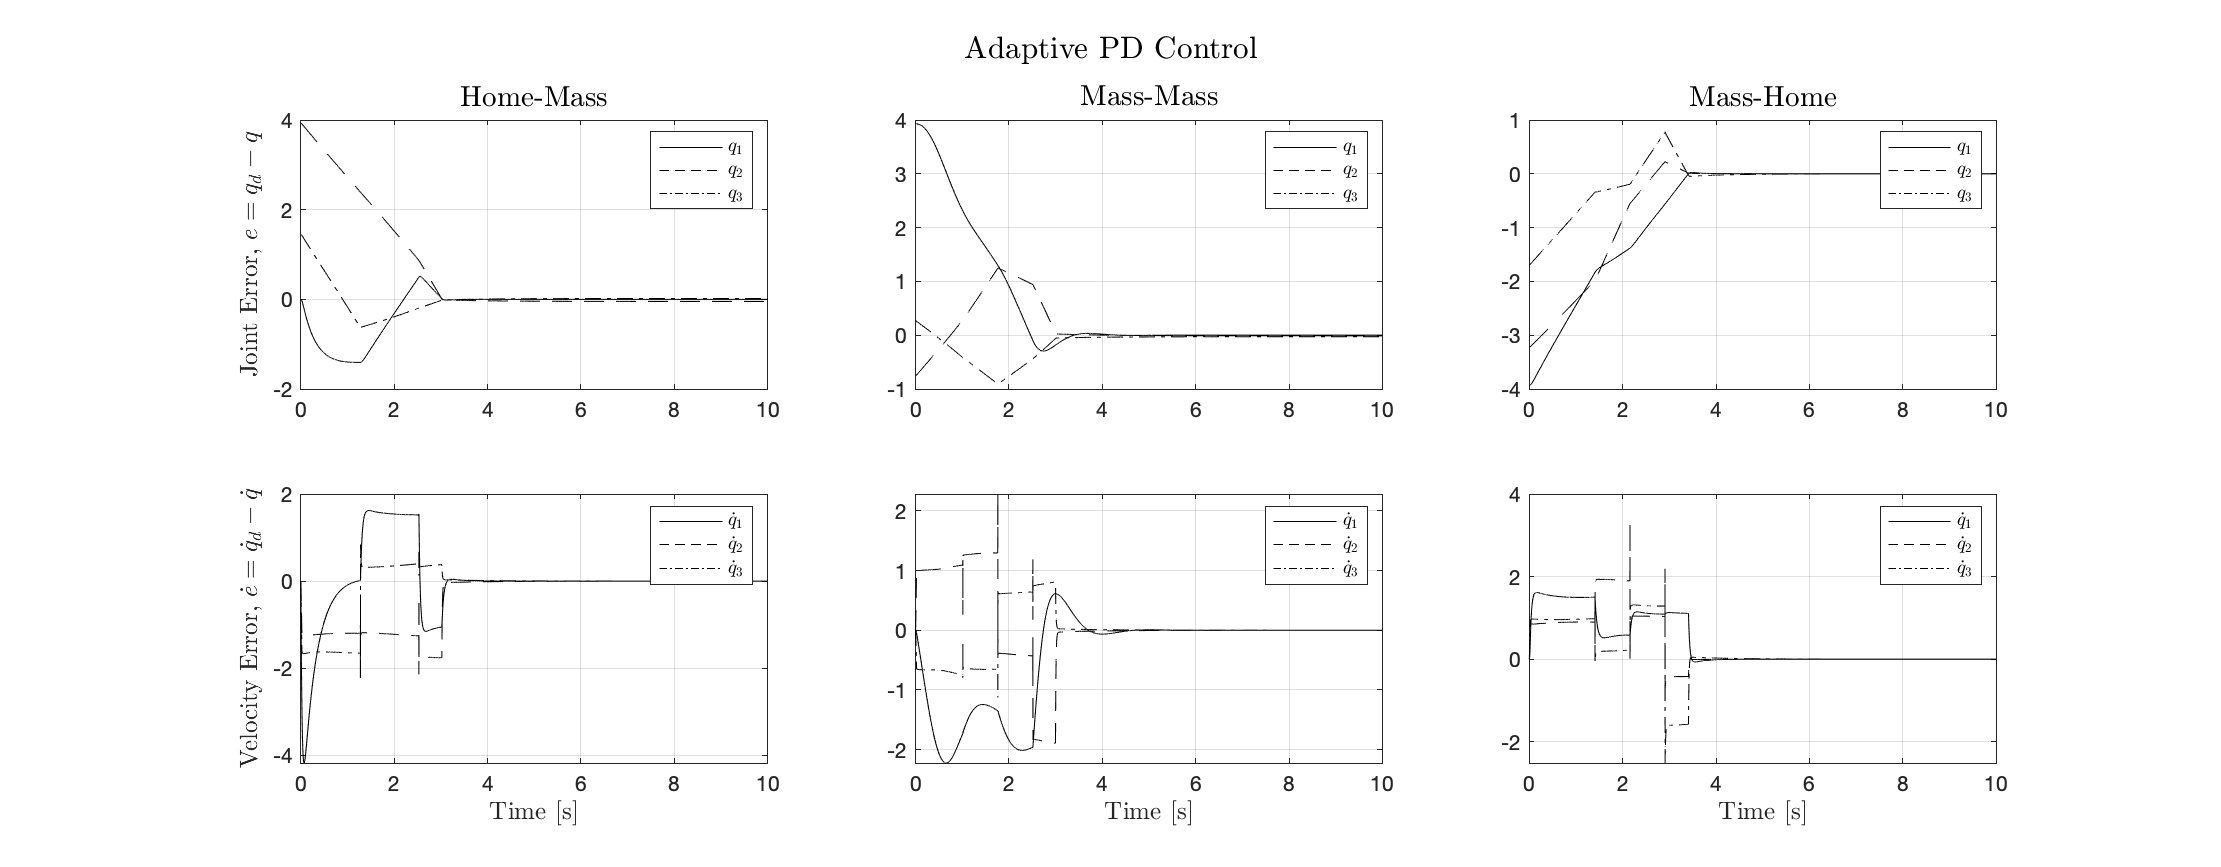
\includegraphics[width=\textwidth]{figures/mass10NNerrAPD.eps}
	\caption{Adaptive controller error in full simulation}
	\label{fig:nnerrapd}
\end{figure}
\begin{figure}[H]
	\centering
	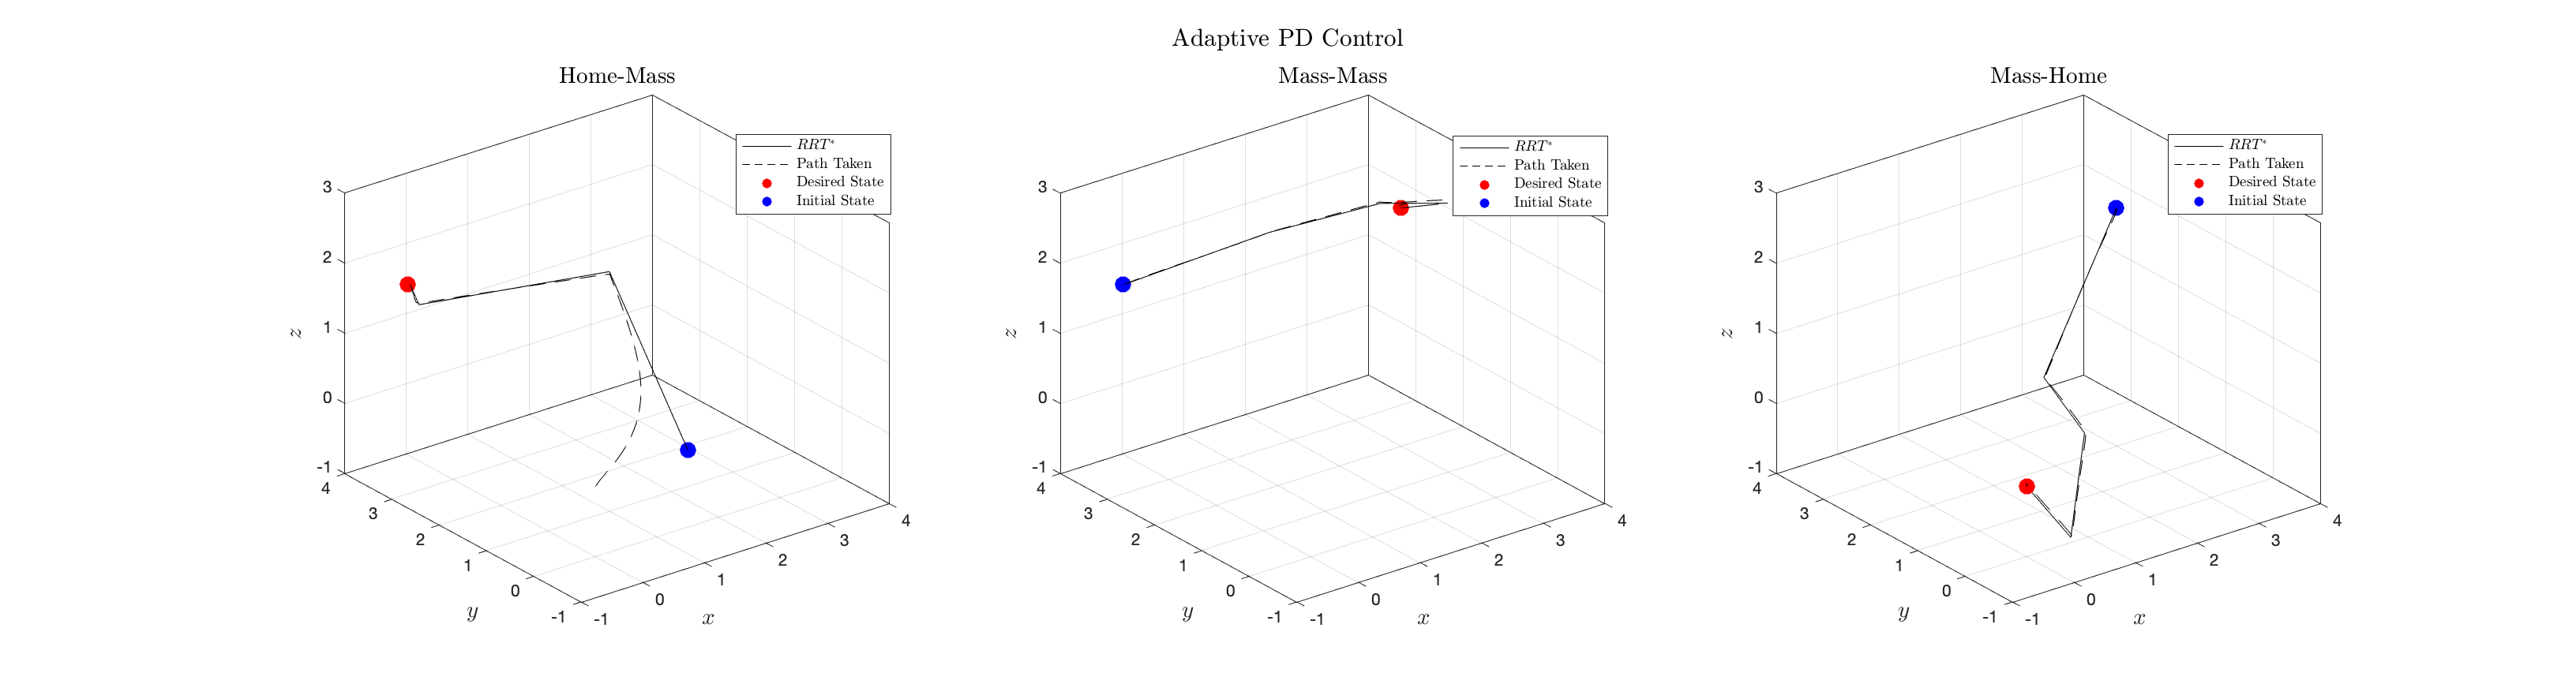
\includegraphics[width=\textwidth]{figures/mass10NNeetrajAPD.eps}
	\caption{End-effector trajectory with adaptive control}
	\label{fig:nntrajapd}
\end{figure}
\noindent We can see from Fig. \ref{fig:nntrajapd} that our initial error results in a false start position, however this error quickly decreases to zero as expected, and the trajectory is followed very tightly for the remainder of the simulation.

We then look at a mass estimated PD model, to observe the effects that an increase in mass has on the control.
\begin{figure}[H]
	\centering
	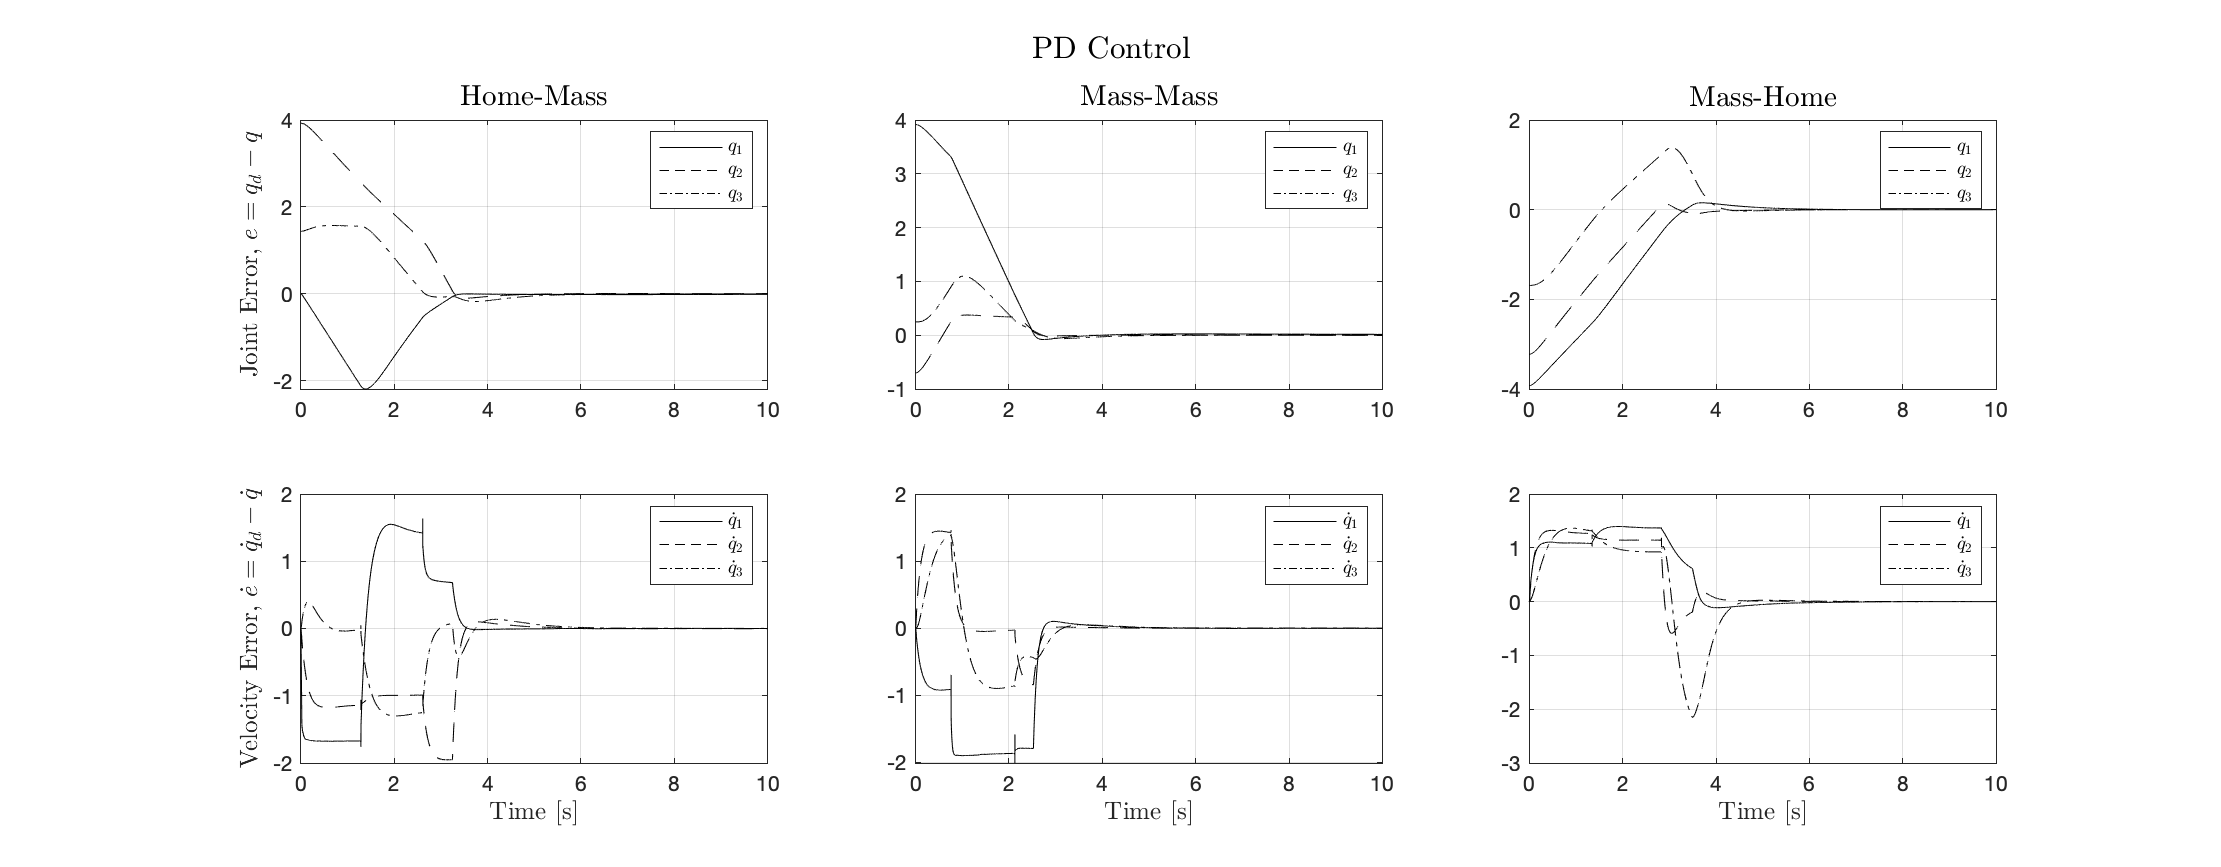
\includegraphics[width=\textwidth]{figures/mass10NNerrPD.eps}
	\caption{Mass estimated PD controller error in full simulation}
	\label{fig:nnerrpd}
\end{figure}
\begin{figure}[H]
	\centering
	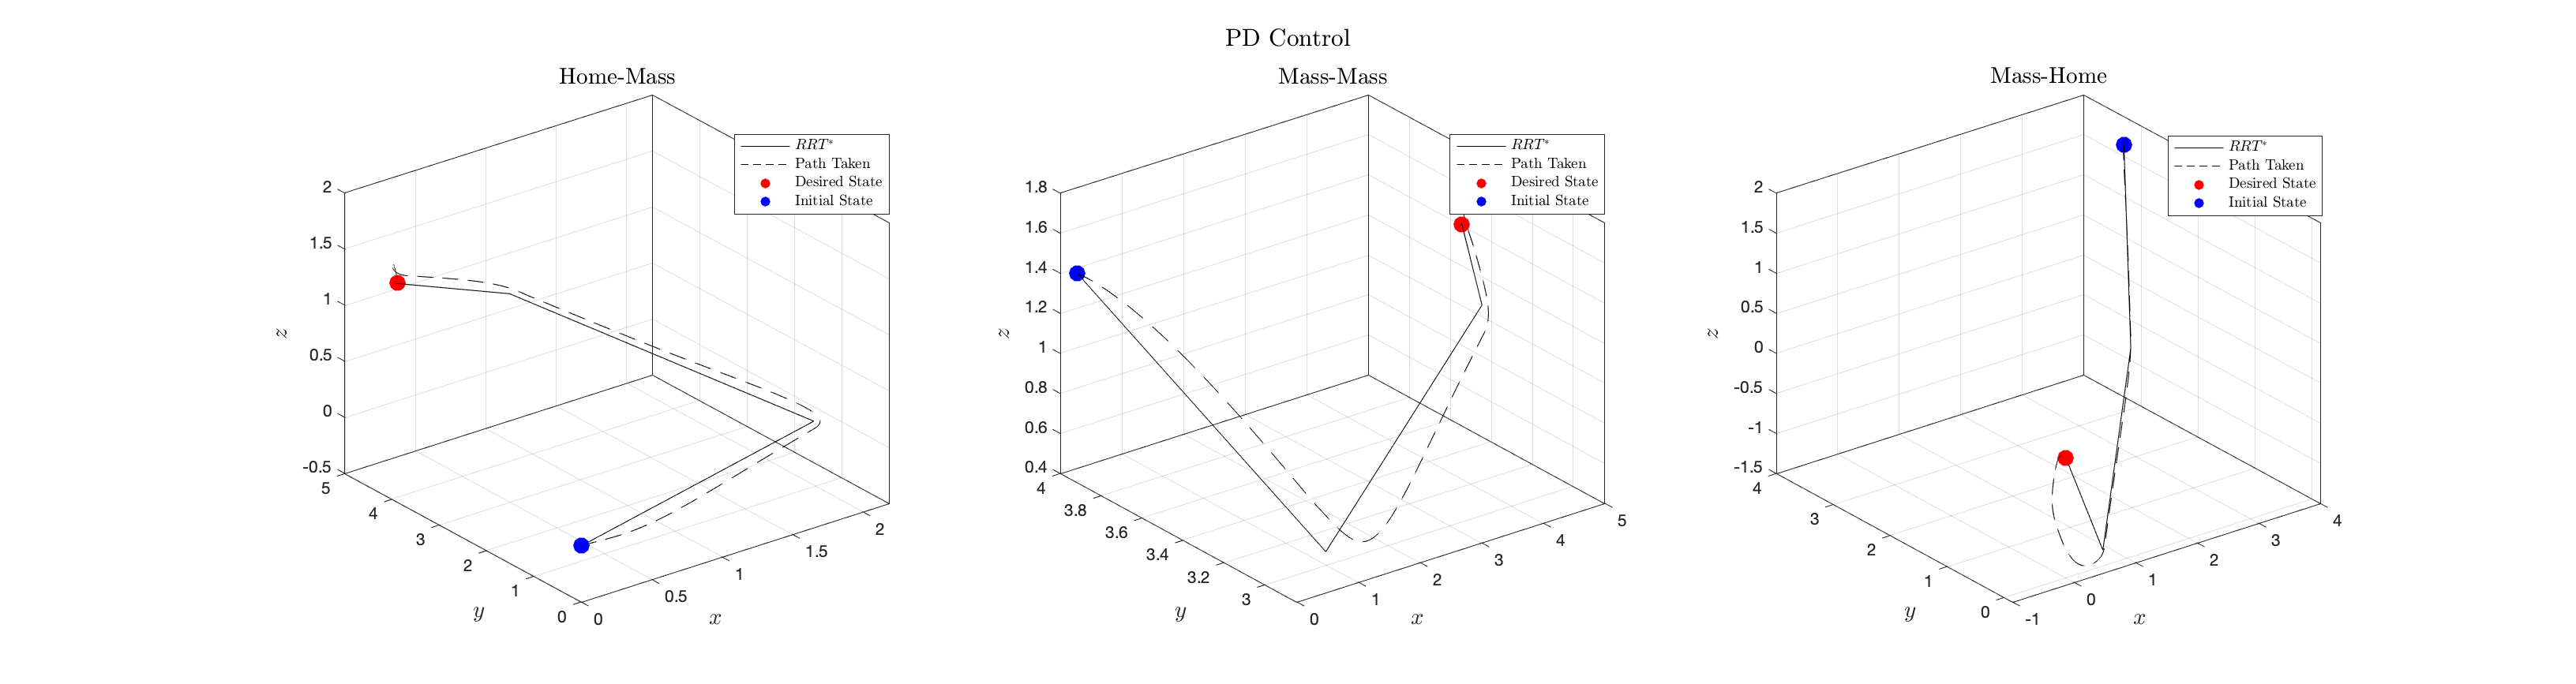
\includegraphics[width=\textwidth]{figures/mass10NNeetrajPD.eps}
	\caption{End-effector trajectory with mass estimated PD control}
	\label{fig:nntrajpd}
\end{figure}
\noindent In contrast to the adaptive model, the mass estimated PD controller places the end-effector in the desired start position.
However, we can easily see from Fig. \ref{fig:nntrajpd} that the PD control is not able to follow the desired trajectory as closely, and once the mass is picked up this issue worsens.


\section{Team Contributions}
For the individual sections of the project, Benton will focus on the robotic
modeling, Ethan on the robotic controls, and Brian on the perception and
tracking.
However, since each part of the project will slowly feed into one another, each
team member will help contribute to all three parts of the project equally.

\end{document}
